% Options for packages loaded elsewhere
\PassOptionsToPackage{unicode}{hyperref}
\PassOptionsToPackage{hyphens}{url}
%
\documentclass[
]{article}
\usepackage{amsmath,amssymb}
\usepackage{lmodern}
\usepackage{iftex}
\ifPDFTeX
  \usepackage[T1]{fontenc}
  \usepackage[utf8]{inputenc}
  \usepackage{textcomp} % provide euro and other symbols
\else % if luatex or xetex
  \usepackage{unicode-math}
  \defaultfontfeatures{Scale=MatchLowercase}
  \defaultfontfeatures[\rmfamily]{Ligatures=TeX,Scale=1}
\fi
% Use upquote if available, for straight quotes in verbatim environments
\IfFileExists{upquote.sty}{\usepackage{upquote}}{}
\IfFileExists{microtype.sty}{% use microtype if available
  \usepackage[]{microtype}
  \UseMicrotypeSet[protrusion]{basicmath} % disable protrusion for tt fonts
}{}
\makeatletter
\@ifundefined{KOMAClassName}{% if non-KOMA class
  \IfFileExists{parskip.sty}{%
    \usepackage{parskip}
  }{% else
    \setlength{\parindent}{0pt}
    \setlength{\parskip}{6pt plus 2pt minus 1pt}}
}{% if KOMA class
  \KOMAoptions{parskip=half}}
\makeatother
\usepackage{xcolor}
\usepackage[margin=1in]{geometry}
\usepackage{color}
\usepackage{fancyvrb}
\newcommand{\VerbBar}{|}
\newcommand{\VERB}{\Verb[commandchars=\\\{\}]}
\DefineVerbatimEnvironment{Highlighting}{Verbatim}{commandchars=\\\{\}}
% Add ',fontsize=\small' for more characters per line
\usepackage{framed}
\definecolor{shadecolor}{RGB}{248,248,248}
\newenvironment{Shaded}{\begin{snugshade}}{\end{snugshade}}
\newcommand{\AlertTok}[1]{\textcolor[rgb]{0.94,0.16,0.16}{#1}}
\newcommand{\AnnotationTok}[1]{\textcolor[rgb]{0.56,0.35,0.01}{\textbf{\textit{#1}}}}
\newcommand{\AttributeTok}[1]{\textcolor[rgb]{0.77,0.63,0.00}{#1}}
\newcommand{\BaseNTok}[1]{\textcolor[rgb]{0.00,0.00,0.81}{#1}}
\newcommand{\BuiltInTok}[1]{#1}
\newcommand{\CharTok}[1]{\textcolor[rgb]{0.31,0.60,0.02}{#1}}
\newcommand{\CommentTok}[1]{\textcolor[rgb]{0.56,0.35,0.01}{\textit{#1}}}
\newcommand{\CommentVarTok}[1]{\textcolor[rgb]{0.56,0.35,0.01}{\textbf{\textit{#1}}}}
\newcommand{\ConstantTok}[1]{\textcolor[rgb]{0.00,0.00,0.00}{#1}}
\newcommand{\ControlFlowTok}[1]{\textcolor[rgb]{0.13,0.29,0.53}{\textbf{#1}}}
\newcommand{\DataTypeTok}[1]{\textcolor[rgb]{0.13,0.29,0.53}{#1}}
\newcommand{\DecValTok}[1]{\textcolor[rgb]{0.00,0.00,0.81}{#1}}
\newcommand{\DocumentationTok}[1]{\textcolor[rgb]{0.56,0.35,0.01}{\textbf{\textit{#1}}}}
\newcommand{\ErrorTok}[1]{\textcolor[rgb]{0.64,0.00,0.00}{\textbf{#1}}}
\newcommand{\ExtensionTok}[1]{#1}
\newcommand{\FloatTok}[1]{\textcolor[rgb]{0.00,0.00,0.81}{#1}}
\newcommand{\FunctionTok}[1]{\textcolor[rgb]{0.00,0.00,0.00}{#1}}
\newcommand{\ImportTok}[1]{#1}
\newcommand{\InformationTok}[1]{\textcolor[rgb]{0.56,0.35,0.01}{\textbf{\textit{#1}}}}
\newcommand{\KeywordTok}[1]{\textcolor[rgb]{0.13,0.29,0.53}{\textbf{#1}}}
\newcommand{\NormalTok}[1]{#1}
\newcommand{\OperatorTok}[1]{\textcolor[rgb]{0.81,0.36,0.00}{\textbf{#1}}}
\newcommand{\OtherTok}[1]{\textcolor[rgb]{0.56,0.35,0.01}{#1}}
\newcommand{\PreprocessorTok}[1]{\textcolor[rgb]{0.56,0.35,0.01}{\textit{#1}}}
\newcommand{\RegionMarkerTok}[1]{#1}
\newcommand{\SpecialCharTok}[1]{\textcolor[rgb]{0.00,0.00,0.00}{#1}}
\newcommand{\SpecialStringTok}[1]{\textcolor[rgb]{0.31,0.60,0.02}{#1}}
\newcommand{\StringTok}[1]{\textcolor[rgb]{0.31,0.60,0.02}{#1}}
\newcommand{\VariableTok}[1]{\textcolor[rgb]{0.00,0.00,0.00}{#1}}
\newcommand{\VerbatimStringTok}[1]{\textcolor[rgb]{0.31,0.60,0.02}{#1}}
\newcommand{\WarningTok}[1]{\textcolor[rgb]{0.56,0.35,0.01}{\textbf{\textit{#1}}}}
\usepackage{graphicx}
\makeatletter
\def\maxwidth{\ifdim\Gin@nat@width>\linewidth\linewidth\else\Gin@nat@width\fi}
\def\maxheight{\ifdim\Gin@nat@height>\textheight\textheight\else\Gin@nat@height\fi}
\makeatother
% Scale images if necessary, so that they will not overflow the page
% margins by default, and it is still possible to overwrite the defaults
% using explicit options in \includegraphics[width, height, ...]{}
\setkeys{Gin}{width=\maxwidth,height=\maxheight,keepaspectratio}
% Set default figure placement to htbp
\makeatletter
\def\fps@figure{htbp}
\makeatother
\setlength{\emergencystretch}{3em} % prevent overfull lines
\providecommand{\tightlist}{%
  \setlength{\itemsep}{0pt}\setlength{\parskip}{0pt}}
\setcounter{secnumdepth}{-\maxdimen} % remove section numbering
\ifLuaTeX
  \usepackage{selnolig}  % disable illegal ligatures
\fi
\IfFileExists{bookmark.sty}{\usepackage{bookmark}}{\usepackage{hyperref}}
\IfFileExists{xurl.sty}{\usepackage{xurl}}{} % add URL line breaks if available
\urlstyle{same} % disable monospaced font for URLs
\hypersetup{
  pdftitle={Mens Boston Marathon Winners},
  pdfauthor={Hilal Özalp},
  hidelinks,
  pdfcreator={LaTeX via pandoc}}

\title{Mens Boston Marathon Winners}
\author{Hilal Özalp}
\date{10.06.2023}

\begin{document}
\maketitle

\#\#\#Excel Tabelle importieren

\begin{Shaded}
\begin{Highlighting}[]
\NormalTok{Mens\_Boston\_Marathon\_Winners }\OtherTok{\textless{}{-}}
  \FunctionTok{read.csv}\NormalTok{(}\StringTok{"C:/Users/Lenovo/Desktop/4.Semsester/Stochastik/R{-}Projekt/Daten/Mens\_Boston\_Marathon\_Winners.csv"}\NormalTok{)}

\CommentTok{\# Libraries setzten}
\FunctionTok{library}\NormalTok{(}\StringTok{"lubridate"}\NormalTok{)}
\end{Highlighting}
\end{Shaded}

\begin{verbatim}
## 
## Attache Paket: 'lubridate'
\end{verbatim}

\begin{verbatim}
## Die folgenden Objekte sind maskiert von 'package:base':
## 
##     date, intersect, setdiff, union
\end{verbatim}

\begin{Shaded}
\begin{Highlighting}[]
\FunctionTok{library}\NormalTok{(}\StringTok{"chron"}\NormalTok{)}
\end{Highlighting}
\end{Shaded}

\begin{verbatim}
## 
## Attache Paket: 'chron'
\end{verbatim}

\begin{verbatim}
## Die folgenden Objekte sind maskiert von 'package:lubridate':
## 
##     days, hours, minutes, seconds, years
\end{verbatim}

\begin{Shaded}
\begin{Highlighting}[]
\FunctionTok{library}\NormalTok{(}\StringTok{"hms"}\NormalTok{)}
\end{Highlighting}
\end{Shaded}

\begin{verbatim}
## 
## Attache Paket: 'hms'
\end{verbatim}

\begin{verbatim}
## Das folgende Objekt ist maskiert 'package:lubridate':
## 
##     hms
\end{verbatim}

\begin{Shaded}
\begin{Highlighting}[]
\FunctionTok{library}\NormalTok{(ggplot2)}
\FunctionTok{library}\NormalTok{(dplyr)}
\end{Highlighting}
\end{Shaded}

\begin{verbatim}
## 
## Attache Paket: 'dplyr'
\end{verbatim}

\begin{verbatim}
## Die folgenden Objekte sind maskiert von 'package:stats':
## 
##     filter, lag
\end{verbatim}

\begin{verbatim}
## Die folgenden Objekte sind maskiert von 'package:base':
## 
##     intersect, setdiff, setequal, union
\end{verbatim}

\#\#\#Durchschnittsdistanz der Männer in km - 41.5693548387097

\begin{Shaded}
\begin{Highlighting}[]
\NormalTok{meanDistanceKm }\OtherTok{\textless{}{-}} \FunctionTok{mean}\NormalTok{(Mens\_Boston\_Marathon\_Winners}\SpecialCharTok{$}\NormalTok{Distance..KM., }\AttributeTok{na.rm =} \ConstantTok{TRUE}\NormalTok{)}
\NormalTok{meanDistanceKm}
\end{Highlighting}
\end{Shaded}

\begin{verbatim}
## [1] 41.56935
\end{verbatim}

\#\#\#Boxplot für die Distanz

\begin{Shaded}
\begin{Highlighting}[]
\FunctionTok{boxplot}\NormalTok{(Mens\_Boston\_Marathon\_Winners}\SpecialCharTok{$}\NormalTok{Distance..KM., }\AttributeTok{main =} \StringTok{"Boxplot für die Distanz"}\NormalTok{, }\AttributeTok{horizontal =} \ConstantTok{TRUE}\NormalTok{)}
\end{Highlighting}
\end{Shaded}

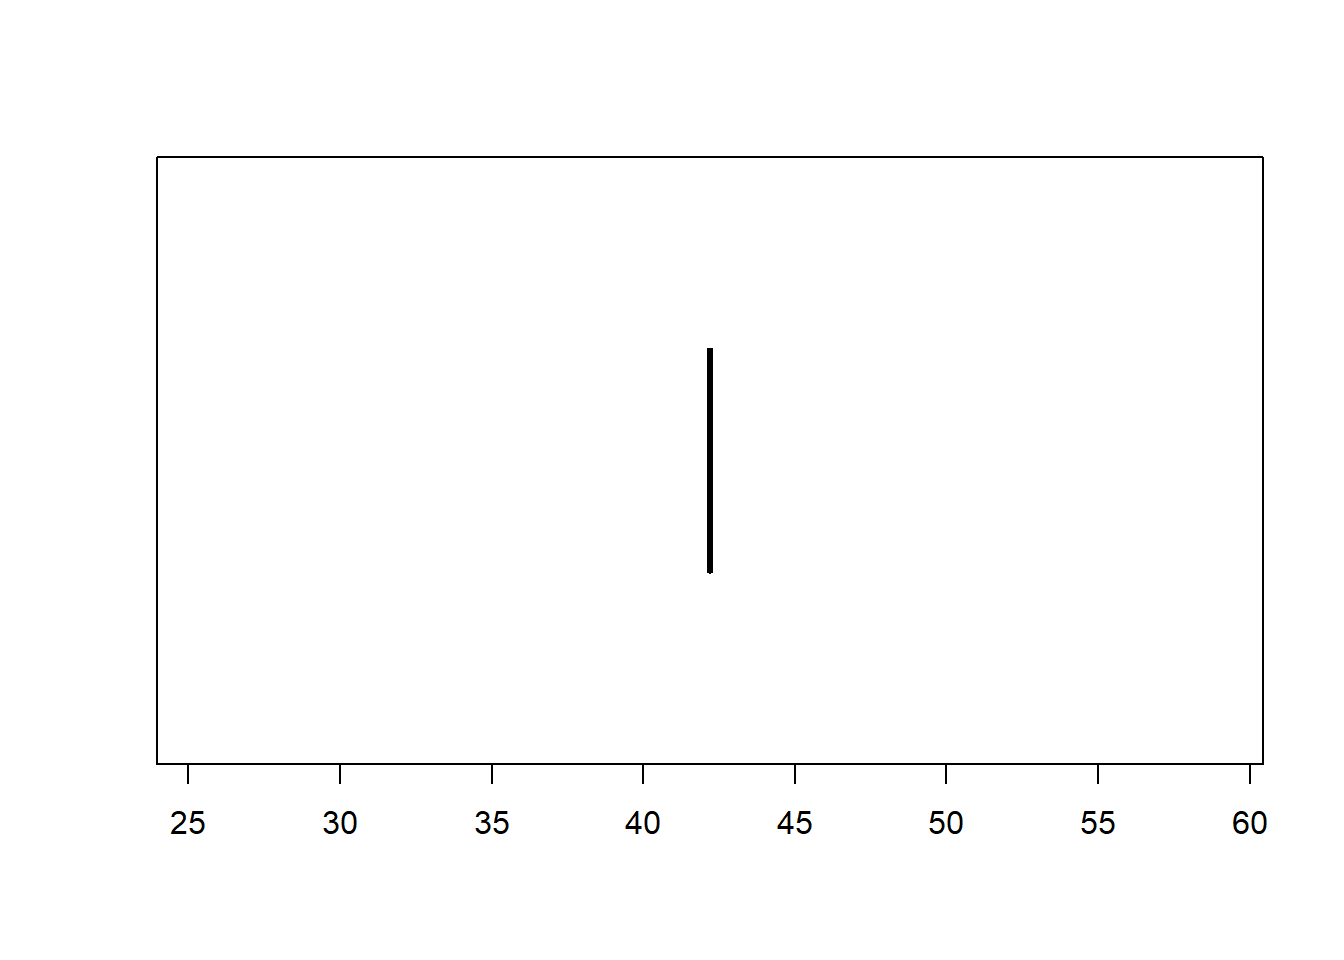
\includegraphics{men_files/figure-latex/unnamed-chunk-3-1.pdf}

Der Boxplot hier macht nicht viel Sinn, da man nicht erkennt wie viele
Läufer welche Distanzen gelaufen sind. Aus diesem Grund eignet sich ein
Balkendiagramm besser, da die Häufigkeit der Distanzen besser zu sehen
sind.

\#\#\#Erstelle ein data.frame für die Distanzzählungen

\begin{Shaded}
\begin{Highlighting}[]
\NormalTok{distance\_counts }\OtherTok{\textless{}{-}} \FunctionTok{table}\NormalTok{(Mens\_Boston\_Marathon\_Winners}\SpecialCharTok{$}\NormalTok{Distance..KM.)}

\NormalTok{df }\OtherTok{\textless{}{-}} \FunctionTok{data.frame}\NormalTok{(}\AttributeTok{Distance =} \FunctionTok{names}\NormalTok{(distance\_counts), }\AttributeTok{Count =} \FunctionTok{as.numeric}\NormalTok{(distance\_counts))}
\NormalTok{df}
\end{Highlighting}
\end{Shaded}

\begin{verbatim}
##   Distance Count
## 1     39.4    26
## 2     41.4     6
## 3       42     3
## 4     42.2    89
\end{verbatim}

\begin{Shaded}
\begin{Highlighting}[]
\CommentTok{\# Erstelle das Balkendiagramm}
\FunctionTok{ggplot}\NormalTok{(df, }\FunctionTok{aes}\NormalTok{(}\AttributeTok{x =}\NormalTok{ Distance, }\AttributeTok{y =}\NormalTok{ Count)) }\SpecialCharTok{+}
  \FunctionTok{geom\_bar}\NormalTok{(}\AttributeTok{stat =} \StringTok{"identity"}\NormalTok{) }\SpecialCharTok{+}
  \FunctionTok{xlab}\NormalTok{(}\StringTok{"Distanz"}\NormalTok{) }\SpecialCharTok{+}
  \FunctionTok{ylab}\NormalTok{(}\StringTok{"Häufigkeit"}\NormalTok{) }\SpecialCharTok{+}
  \FunctionTok{ggtitle}\NormalTok{(}\StringTok{"Häufigkeit der Distanzen"}\NormalTok{) }\SpecialCharTok{+}
  \FunctionTok{theme}\NormalTok{(}\AttributeTok{axis.text.x =} \FunctionTok{element\_text}\NormalTok{(}\AttributeTok{angle =} \DecValTok{45}\NormalTok{, }\AttributeTok{hjust =} \DecValTok{1}\NormalTok{))}
\end{Highlighting}
\end{Shaded}

\includegraphics{men_files/figure-latex/unnamed-chunk-4-1.pdf}

\#\#\#Durchschnittszeit der Männer - 02:21:31

\begin{Shaded}
\begin{Highlighting}[]
\NormalTok{meanTime }\OtherTok{\textless{}{-}} \FunctionTok{mean}\NormalTok{(}\FunctionTok{times}\NormalTok{(Mens\_Boston\_Marathon\_Winners}\SpecialCharTok{$}\NormalTok{Time))}
\NormalTok{meanTime}
\end{Highlighting}
\end{Shaded}

\begin{verbatim}
## [1] 02:21:31
\end{verbatim}

\#DurchschnittsGeschwindigkeit der Männer - 3 min 24 sek

\begin{Shaded}
\begin{Highlighting}[]
\NormalTok{meanSpeed }\OtherTok{\textless{}{-}}\NormalTok{ meanTime}\SpecialCharTok{/}\NormalTok{meanDistanceKm}
\NormalTok{meanSpeed}
\end{Highlighting}
\end{Shaded}

\begin{verbatim}
## [1] 00:03:24
\end{verbatim}

\#Boxplot für die Durchschnittgeschwindigkeit

\begin{Shaded}
\begin{Highlighting}[]
\CommentTok{\# Geschwindigkeiten von den einzelnen Männern}
\NormalTok{men\_times }\OtherTok{\textless{}{-}} \FunctionTok{format}\NormalTok{(}\FunctionTok{as.POSIXct}\NormalTok{(}\FunctionTok{strptime}\NormalTok{(Mens\_Boston\_Marathon\_Winners}\SpecialCharTok{$}\NormalTok{Time, }\AttributeTok{format=}\StringTok{"\%H:\%M:\%S"}\NormalTok{)), }
                    \AttributeTok{format =} \StringTok{"\%H:\%M:\%S"}\NormalTok{)}
\NormalTok{men\_times\_hms }\OtherTok{\textless{}{-}} \FunctionTok{as\_hms}\NormalTok{(men\_times) }\CommentTok{\# Umwandlung in Stunden{-}Minuten{-}Sekunden}
\NormalTok{men\_times\_in\_seconds }\OtherTok{\textless{}{-}}\NormalTok{ lubridate}\SpecialCharTok{::}\FunctionTok{seconds}\NormalTok{(men\_times\_hms)}
\NormalTok{men\_times\_in\_minutes }\OtherTok{\textless{}{-}} \FunctionTok{as.numeric}\NormalTok{(men\_times\_in\_seconds }\SpecialCharTok{/} \DecValTok{60}\NormalTok{)}
\NormalTok{men\_speeds }\OtherTok{\textless{}{-}}\NormalTok{ men\_times\_in\_minutes }\SpecialCharTok{/}\NormalTok{ Mens\_Boston\_Marathon\_Winners}\SpecialCharTok{$}\NormalTok{Distance..KM.}
\NormalTok{men\_speeds}
\end{Highlighting}
\end{Shaded}

\begin{verbatim}
##   [1] 4.445854 4.111675 4.432318 4.054146 3.791455 4.142132 4.098562 4.011844
##   [9] 4.020728 4.206853 3.664975 3.698393 4.406091 3.778342 3.595178 3.586294
##  [17] 3.686125 3.686125 3.849831 3.737733 3.771997       NA 3.787225 3.794839
##  [25] 3.526650 3.506768 3.649323 3.563492 3.642857 3.468254 3.800158 3.723144
##  [33] 3.628752 3.668246 3.951422 3.639810 3.578594 3.622828 3.604660 3.641390
##  [41] 3.633491 3.686414 3.527251 3.518167 3.569510 3.479858 3.516983 3.597946
##  [49] 3.570300 3.541469 3.451422 3.578989 3.597946 3.617299 3.568841 3.668680
##  [57] 3.353865 3.397343 3.342190 3.242351 3.319510 3.457346 3.381517 3.338863
##  [65] 3.404028 3.407583 3.293049 3.317141 3.235782 3.250790 3.216825 3.371643
##  [73] 3.171011 3.092417 3.287915 3.214455 3.223934 3.167062 3.078594 3.325039
##  [81] 3.193523 3.085703 3.067536 3.132306 3.067141 3.053712 3.056872 3.093997
##  [89] 3.177330 3.029621 3.124013 3.050158 3.059242 3.040679 3.106635 3.038705
##  [97] 3.069905 3.015403 3.065561 3.062796 3.093997 3.022907 3.077409 3.075434
## [105] 3.073855 3.057662 3.084913 3.095182 3.121643 3.015008 3.180490 3.027251
## [113] 3.049763 2.982622 2.915482 3.143760 3.089258 3.047788 3.063586 3.145735
## [121] 3.071485 3.221959 3.031991       NA 3.077014 3.005924
\end{verbatim}

\begin{Shaded}
\begin{Highlighting}[]
\CommentTok{\# Boxplot für men\_speeds erstellen}
\FunctionTok{boxplot}\NormalTok{(men\_speeds, }\AttributeTok{main =} \StringTok{"Boxplot für Geschwindigkeiten der Männer"}\NormalTok{, }\AttributeTok{xlab =} \StringTok{"Geschwindigkeit (Minuten pro Kilometer)"}\NormalTok{, }\AttributeTok{horizontal =} \ConstantTok{TRUE}\NormalTok{)}
\end{Highlighting}
\end{Shaded}

\includegraphics{men_files/figure-latex/unnamed-chunk-7-1.pdf}

\#\#\#Boxplot für die Zeit

\begin{Shaded}
\begin{Highlighting}[]
\NormalTok{timeData }\OtherTok{\textless{}{-}} \FunctionTok{times}\NormalTok{(Mens\_Boston\_Marathon\_Winners}\SpecialCharTok{$}\NormalTok{Time)}

\FunctionTok{boxplot}\NormalTok{(timeData,}
        \AttributeTok{main =}\StringTok{"Boston Marathon Winners (Men)"}\NormalTok{,}
        \AttributeTok{xlab =}\StringTok{"Time"}\NormalTok{,}
        \AttributeTok{col =} \StringTok{"lightblue"}\NormalTok{,}
        \AttributeTok{horizontal =} \ConstantTok{TRUE}\NormalTok{)}
\end{Highlighting}
\end{Shaded}

\includegraphics{men_files/figure-latex/unnamed-chunk-8-1.pdf}

\#\#\#Gewinneranzahl pro Land

\begin{Shaded}
\begin{Highlighting}[]
\NormalTok{frequency }\OtherTok{\textless{}{-}} \FunctionTok{table}\NormalTok{(Mens\_Boston\_Marathon\_Winners}\SpecialCharTok{$}\NormalTok{Country, }\AttributeTok{exclude =} \FunctionTok{c}\NormalTok{(}\ConstantTok{NULL}\NormalTok{, }\StringTok{""}\NormalTok{))}
\NormalTok{country\_df }\OtherTok{\textless{}{-}} \FunctionTok{data.frame}\NormalTok{(}\AttributeTok{Land =} \FunctionTok{names}\NormalTok{(frequency), Häufigkeit }\OtherTok{=} \FunctionTok{as.vector}\NormalTok{(}\FunctionTok{unname}\NormalTok{(frequency)))}
\NormalTok{country\_df }\OtherTok{\textless{}{-}} \FunctionTok{arrange}\NormalTok{(country\_df, }\FunctionTok{desc}\NormalTok{(frequency))}
\NormalTok{country\_df}
\end{Highlighting}
\end{Shaded}

\begin{verbatim}
##              Land Häufigkeit
## 1   United States         43
## 2           Kenya         24
## 3          Canada         16
## 4           Japan          9
## 5         Finland          7
## 6        Ethiopia          6
## 7     South Korea          3
## 8  United Kingdom          3
## 9         Belgium          2
## 10         Greece          2
## 11      Australia          1
## 12       Colombia          1
## 13        Germany          1
## 14      Guatemala          1
## 15        Ireland          1
## 16          Italy          1
## 17    New Zealand          1
## 18         Sweden          1
## 19     Yugoslavia          1
\end{verbatim}

\begin{Shaded}
\begin{Highlighting}[]
\CommentTok{\# Abgekürzte Ländernamen erstellen}
\NormalTok{abbreviated\_names }\OtherTok{\textless{}{-}} \FunctionTok{abbreviate}\NormalTok{(country\_df}\SpecialCharTok{$}\NormalTok{Land, }\AttributeTok{minlength =} \DecValTok{10}\NormalTok{)}

\CommentTok{\# Säulendiagramm mit abgekürzten Ländernamen erstellen}
\FunctionTok{barplot}\NormalTok{(country\_df}\SpecialCharTok{$}\NormalTok{Häufigkeit, }\AttributeTok{main =} \StringTok{"Säulendiagramm für Länder{-}Häufigkeit"}\NormalTok{,}
        \AttributeTok{xlab =} \StringTok{"Land"}\NormalTok{, }\AttributeTok{ylab =} \StringTok{"Häufigkeit"}\NormalTok{, }\AttributeTok{cex.names =} \FloatTok{0.8}\NormalTok{, }\AttributeTok{ylim =} \FunctionTok{c}\NormalTok{(}\DecValTok{0}\NormalTok{, }\FunctionTok{max}\NormalTok{(country\_df}\SpecialCharTok{$}\NormalTok{Häufigkeit) }\SpecialCharTok{+} \DecValTok{1}\NormalTok{), }
        \AttributeTok{las =} \DecValTok{2}\NormalTok{, }\AttributeTok{cex.axis =} \FloatTok{0.8}\NormalTok{, }\AttributeTok{cex.lab =} \FloatTok{0.8}\NormalTok{, }\AttributeTok{width =} \FloatTok{0.8}\NormalTok{, }\AttributeTok{space =} \FloatTok{0.5}\NormalTok{, }\AttributeTok{names.arg =}\NormalTok{ abbreviated\_names)}
\end{Highlighting}
\end{Shaded}

\includegraphics{men_files/figure-latex/unnamed-chunk-9-1.pdf} Ergebnis
des Balkendiagramms: Die meisten Gewinner kommen aus den USA mit 43,
gefolgt von Kenya mit 24 und Canada mit 16

\#Vergleich der Geschwindigkeiten und Entfernung

\begin{Shaded}
\begin{Highlighting}[]
\CommentTok{\# Erstelle ein data.frame mit den Jahreszahlen, Zeit und Distanz}
\NormalTok{df }\OtherTok{\textless{}{-}} \FunctionTok{data.frame}\NormalTok{(}\AttributeTok{Jahr =}\NormalTok{ Mens\_Boston\_Marathon\_Winners}\SpecialCharTok{$}\NormalTok{Year, }\AttributeTok{Zeit =} \FunctionTok{times}\NormalTok{(Mens\_Boston\_Marathon\_Winners}\SpecialCharTok{$}\NormalTok{Time), }\AttributeTok{Distanz =}\NormalTok{ Mens\_Boston\_Marathon\_Winners}\SpecialCharTok{$}\NormalTok{Distance..KM.)}

\NormalTok{df}
\end{Highlighting}
\end{Shaded}

\begin{verbatim}
##     Jahr     Zeit Distanz
## 1   1897 02:55:10    39.4
## 2   1898 02:42:00    39.4
## 3   1899 02:54:38    39.4
## 4   1900 02:39:44    39.4
## 5   1901 02:29:23    39.4
## 6   1902 02:43:12    39.4
## 7   1903 02:41:29    39.4
## 8   1904 02:38:04    39.4
## 9   1905 02:38:25    39.4
## 10  1906 02:45:45    39.4
## 11  1907 02:24:24    39.4
## 12  1908 02:25:43    39.4
## 13  1909 02:53:36    39.4
## 14  1910 02:28:52    39.4
## 15  1911 02:21:39    39.4
## 16  1912 02:21:18    39.4
## 17  1913 02:25:14    39.4
## 18  1914 02:25:14    39.4
## 19  1915 02:31:41    39.4
## 20  1916 02:27:16    39.4
## 21  1917 02:28:37    39.4
## 22    NA     <NA>      NA
## 23  1919 02:29:13    39.4
## 24  1920 02:29:31    39.4
## 25  1921 02:18:57    39.4
## 26  1922 02:18:10    39.4
## 27  1923 02:23:47    39.4
## 28  1924 02:29:40    42.0
## 29  1925 02:33:00    42.0
## 30  1926 02:25:40    42.0
## 31  1927 02:40:22    42.2
## 32  1928 02:37:07    42.2
## 33  1929 02:33:08    42.2
## 34  1930 02:34:48    42.2
## 35  1931 02:46:45    42.2
## 36  1932 02:33:36    42.2
## 37  1933 02:31:01    42.2
## 38  1934 02:32:53    42.2
## 39  1935 02:32:07    42.2
## 40  1936 02:33:40    42.2
## 41  1937 02:33:20    42.2
## 42  1938 02:35:34    42.2
## 43  1939 02:28:51    42.2
## 44  1940 02:28:28    42.2
## 45  1941 02:30:38    42.2
## 46  1942 02:26:51    42.2
## 47  1943 02:28:25    42.2
## 48  1944 02:31:50    42.2
## 49  1945 02:30:40    42.2
## 50  1946 02:29:27    42.2
## 51  1947 02:25:39    42.2
## 52  1948 02:31:02    42.2
## 53  1949 02:31:50    42.2
## 54  1950 02:32:39    42.2
## 55  1951 02:27:45    41.4
## 56  1952 02:31:53    41.4
## 57  1953 02:18:51    41.4
## 58  1954 02:20:39    41.4
## 59  1955 02:18:22    41.4
## 60  1956 02:14:14    41.4
## 61  1957 02:20:05    42.2
## 62  1958 02:25:54    42.2
## 63  1959 02:22:42    42.2
## 64  1960 02:20:54    42.2
## 65  1961 02:23:39    42.2
## 66  1962 02:23:48    42.2
## 67  1963 02:18:58    42.2
## 68  1964 02:19:59    42.2
## 69  1965 02:16:33    42.2
## 70  1966 02:17:11    42.2
## 71  1967 02:15:45    42.2
## 72  1968 02:22:17    42.2
## 73  1969 02:13:49    42.2
## 74  1970 02:10:30    42.2
## 75  1971 02:18:45    42.2
## 76  1972 02:15:39    42.2
## 77  1973 02:16:03    42.2
## 78  1974 02:13:39    42.2
## 79  1975 02:09:55    42.2
## 80  1976 02:20:19    42.2
## 81  1977 02:14:46    42.2
## 82  1978 02:10:13    42.2
## 83  1979 02:09:27    42.2
## 84  1980 02:12:11    42.2
## 85  1981 02:09:26    42.2
## 86  1982 02:08:52    42.2
## 87  1983 02:09:00    42.2
## 88  1984 02:10:34    42.2
## 89  1985 02:14:05    42.2
## 90  1986 02:07:51    42.2
## 91  1987 02:11:50    42.2
## 92  1988 02:08:43    42.2
## 93  1989 02:09:06    42.2
## 94  1990 02:08:19    42.2
## 95  1991 02:11:06    42.2
## 96  1992 02:08:14    42.2
## 97  1993 02:09:33    42.2
## 98  1994 02:07:15    42.2
## 99  1995 02:09:22    42.2
## 100 1996 02:09:15    42.2
## 101 1997 02:10:34    42.2
## 102 1998 02:07:34    42.2
## 103 1999 02:09:52    42.2
## 104 2000 02:09:47    42.2
## 105 2001 02:09:43    42.2
## 106 2002 02:09:02    42.2
## 107 2003 02:10:11    42.2
## 108 2004 02:10:37    42.2
## 109 2005 02:11:44    42.2
## 110 2006 02:07:14    42.2
## 111 2007 02:14:13    42.2
## 112 2008 02:07:45    42.2
## 113 2009 02:08:42    42.2
## 114 2010 02:05:52    42.2
## 115 2011 02:03:02    42.2
## 116 2012 02:12:40    42.2
## 117 2013 02:10:22    42.2
## 118 2014 02:08:37    42.2
## 119 2015 02:09:17    42.2
## 120 2016 02:12:45    42.2
## 121 2017 02:09:37    42.2
## 122 2018 02:15:58    42.2
## 123 2019 02:07:57    42.2
## 124   NA     <NA>      NA
## 125 2021 02:09:51    42.2
## 126 2022 02:06:51    42.2
\end{verbatim}

\begin{Shaded}
\begin{Highlighting}[]
\CommentTok{\#Geschwindigkeit berechnen und anschließend und hinzufügen}
\CommentTok{\# Geschwindigkeiten von Männern}
\NormalTok{men\_times }\OtherTok{\textless{}{-}} \FunctionTok{format}\NormalTok{(}\FunctionTok{as.POSIXct}\NormalTok{(}\FunctionTok{strptime}\NormalTok{(Mens\_Boston\_Marathon\_Winners}\SpecialCharTok{$}\NormalTok{Time, }\AttributeTok{format=}\StringTok{"\%H:\%M:\%S"}\NormalTok{)), }
                    \AttributeTok{format =} \StringTok{"\%H:\%M:\%S"}\NormalTok{)}
\NormalTok{men\_times\_hms }\OtherTok{\textless{}{-}} \FunctionTok{as\_hms}\NormalTok{(men\_times) }\CommentTok{\# Umwandlung in Stunden{-}Minuten{-}Sekunden}
\NormalTok{men\_times\_in\_seconds }\OtherTok{\textless{}{-}}\NormalTok{ lubridate}\SpecialCharTok{::}\FunctionTok{seconds}\NormalTok{(men\_times\_hms)}
\NormalTok{men\_times\_in\_minutes }\OtherTok{\textless{}{-}} \FunctionTok{as.numeric}\NormalTok{(men\_times\_in\_seconds }\SpecialCharTok{/} \DecValTok{60}\NormalTok{)}
\NormalTok{men\_speeds }\OtherTok{\textless{}{-}}\NormalTok{ men\_times\_in\_minutes }\SpecialCharTok{/}\NormalTok{ Mens\_Boston\_Marathon\_Winners}\SpecialCharTok{$}\NormalTok{Distance..KM.}

\NormalTok{df }\OtherTok{\textless{}{-}} \FunctionTok{data.frame}\NormalTok{(df, }\AttributeTok{Geschwindigkeit =}\NormalTok{ men\_speeds)}
\NormalTok{df}
\end{Highlighting}
\end{Shaded}

\begin{verbatim}
##     Jahr     Zeit Distanz Geschwindigkeit
## 1   1897 02:55:10    39.4        4.445854
## 2   1898 02:42:00    39.4        4.111675
## 3   1899 02:54:38    39.4        4.432318
## 4   1900 02:39:44    39.4        4.054146
## 5   1901 02:29:23    39.4        3.791455
## 6   1902 02:43:12    39.4        4.142132
## 7   1903 02:41:29    39.4        4.098562
## 8   1904 02:38:04    39.4        4.011844
## 9   1905 02:38:25    39.4        4.020728
## 10  1906 02:45:45    39.4        4.206853
## 11  1907 02:24:24    39.4        3.664975
## 12  1908 02:25:43    39.4        3.698393
## 13  1909 02:53:36    39.4        4.406091
## 14  1910 02:28:52    39.4        3.778342
## 15  1911 02:21:39    39.4        3.595178
## 16  1912 02:21:18    39.4        3.586294
## 17  1913 02:25:14    39.4        3.686125
## 18  1914 02:25:14    39.4        3.686125
## 19  1915 02:31:41    39.4        3.849831
## 20  1916 02:27:16    39.4        3.737733
## 21  1917 02:28:37    39.4        3.771997
## 22    NA     <NA>      NA              NA
## 23  1919 02:29:13    39.4        3.787225
## 24  1920 02:29:31    39.4        3.794839
## 25  1921 02:18:57    39.4        3.526650
## 26  1922 02:18:10    39.4        3.506768
## 27  1923 02:23:47    39.4        3.649323
## 28  1924 02:29:40    42.0        3.563492
## 29  1925 02:33:00    42.0        3.642857
## 30  1926 02:25:40    42.0        3.468254
## 31  1927 02:40:22    42.2        3.800158
## 32  1928 02:37:07    42.2        3.723144
## 33  1929 02:33:08    42.2        3.628752
## 34  1930 02:34:48    42.2        3.668246
## 35  1931 02:46:45    42.2        3.951422
## 36  1932 02:33:36    42.2        3.639810
## 37  1933 02:31:01    42.2        3.578594
## 38  1934 02:32:53    42.2        3.622828
## 39  1935 02:32:07    42.2        3.604660
## 40  1936 02:33:40    42.2        3.641390
## 41  1937 02:33:20    42.2        3.633491
## 42  1938 02:35:34    42.2        3.686414
## 43  1939 02:28:51    42.2        3.527251
## 44  1940 02:28:28    42.2        3.518167
## 45  1941 02:30:38    42.2        3.569510
## 46  1942 02:26:51    42.2        3.479858
## 47  1943 02:28:25    42.2        3.516983
## 48  1944 02:31:50    42.2        3.597946
## 49  1945 02:30:40    42.2        3.570300
## 50  1946 02:29:27    42.2        3.541469
## 51  1947 02:25:39    42.2        3.451422
## 52  1948 02:31:02    42.2        3.578989
## 53  1949 02:31:50    42.2        3.597946
## 54  1950 02:32:39    42.2        3.617299
## 55  1951 02:27:45    41.4        3.568841
## 56  1952 02:31:53    41.4        3.668680
## 57  1953 02:18:51    41.4        3.353865
## 58  1954 02:20:39    41.4        3.397343
## 59  1955 02:18:22    41.4        3.342190
## 60  1956 02:14:14    41.4        3.242351
## 61  1957 02:20:05    42.2        3.319510
## 62  1958 02:25:54    42.2        3.457346
## 63  1959 02:22:42    42.2        3.381517
## 64  1960 02:20:54    42.2        3.338863
## 65  1961 02:23:39    42.2        3.404028
## 66  1962 02:23:48    42.2        3.407583
## 67  1963 02:18:58    42.2        3.293049
## 68  1964 02:19:59    42.2        3.317141
## 69  1965 02:16:33    42.2        3.235782
## 70  1966 02:17:11    42.2        3.250790
## 71  1967 02:15:45    42.2        3.216825
## 72  1968 02:22:17    42.2        3.371643
## 73  1969 02:13:49    42.2        3.171011
## 74  1970 02:10:30    42.2        3.092417
## 75  1971 02:18:45    42.2        3.287915
## 76  1972 02:15:39    42.2        3.214455
## 77  1973 02:16:03    42.2        3.223934
## 78  1974 02:13:39    42.2        3.167062
## 79  1975 02:09:55    42.2        3.078594
## 80  1976 02:20:19    42.2        3.325039
## 81  1977 02:14:46    42.2        3.193523
## 82  1978 02:10:13    42.2        3.085703
## 83  1979 02:09:27    42.2        3.067536
## 84  1980 02:12:11    42.2        3.132306
## 85  1981 02:09:26    42.2        3.067141
## 86  1982 02:08:52    42.2        3.053712
## 87  1983 02:09:00    42.2        3.056872
## 88  1984 02:10:34    42.2        3.093997
## 89  1985 02:14:05    42.2        3.177330
## 90  1986 02:07:51    42.2        3.029621
## 91  1987 02:11:50    42.2        3.124013
## 92  1988 02:08:43    42.2        3.050158
## 93  1989 02:09:06    42.2        3.059242
## 94  1990 02:08:19    42.2        3.040679
## 95  1991 02:11:06    42.2        3.106635
## 96  1992 02:08:14    42.2        3.038705
## 97  1993 02:09:33    42.2        3.069905
## 98  1994 02:07:15    42.2        3.015403
## 99  1995 02:09:22    42.2        3.065561
## 100 1996 02:09:15    42.2        3.062796
## 101 1997 02:10:34    42.2        3.093997
## 102 1998 02:07:34    42.2        3.022907
## 103 1999 02:09:52    42.2        3.077409
## 104 2000 02:09:47    42.2        3.075434
## 105 2001 02:09:43    42.2        3.073855
## 106 2002 02:09:02    42.2        3.057662
## 107 2003 02:10:11    42.2        3.084913
## 108 2004 02:10:37    42.2        3.095182
## 109 2005 02:11:44    42.2        3.121643
## 110 2006 02:07:14    42.2        3.015008
## 111 2007 02:14:13    42.2        3.180490
## 112 2008 02:07:45    42.2        3.027251
## 113 2009 02:08:42    42.2        3.049763
## 114 2010 02:05:52    42.2        2.982622
## 115 2011 02:03:02    42.2        2.915482
## 116 2012 02:12:40    42.2        3.143760
## 117 2013 02:10:22    42.2        3.089258
## 118 2014 02:08:37    42.2        3.047788
## 119 2015 02:09:17    42.2        3.063586
## 120 2016 02:12:45    42.2        3.145735
## 121 2017 02:09:37    42.2        3.071485
## 122 2018 02:15:58    42.2        3.221959
## 123 2019 02:07:57    42.2        3.031991
## 124   NA     <NA>      NA              NA
## 125 2021 02:09:51    42.2        3.077014
## 126 2022 02:06:51    42.2        3.005924
\end{verbatim}

\begin{Shaded}
\begin{Highlighting}[]
\CommentTok{\# Erstelle Streudiagramm}
\FunctionTok{plot}\NormalTok{(df}\SpecialCharTok{$}\NormalTok{Geschwindigkeit, df}\SpecialCharTok{$}\NormalTok{Distanz, }\AttributeTok{xlab =} \StringTok{"Geschwindigkeit"}\NormalTok{, }\AttributeTok{ylab =} \StringTok{"Distanz"}\NormalTok{, }\AttributeTok{main =}\StringTok{"Vergleich zwischen der Geschwindigkeit und der Entfernung"}\NormalTok{)}
\end{Highlighting}
\end{Shaded}

\includegraphics{men_files/figure-latex/unnamed-chunk-10-1.pdf} Man
sieht, dass man beim 42.2 Marathon ca. bei ca 3.1 min/km eine Häufung
hat - Die läufer waran beim längeren Marathon laut Streudiagramm
schneller als bei den anderen.

\end{document}
